\documentclass{beamer}

\usepackage[utf8]{inputenc}
\usepackage[T1]{fontenc}
\usepackage[french]{babel}
\usepackage[babel=true]{csquotes} % guillements français
\usepackage{graphicx}
\graphicspath{{Images/}{Images/L3_Android/}}
\usepackage{color}
\usepackage{hyperref}
\hypersetup{colorlinks,linkcolor=,urlcolor=blue}
\usepackage{float}
\usepackage[lined,boxed,commentsnumbered, ruled,vlined,linesnumbered, french, frenchkw, onelanguage]{algorithm2e}
\SetAlFnt{\tiny}
\usepackage{pgffor}
\usepackage[normalem]{ulem}
\usepackage{minted}
\usepackage{schemabloc}
\usepackage{mathtools}

\newcommand{\N}{\mathbb{N}}
\newcommand{\R}{\mathbb{R}}
\newcommand{\Min}[1]{\min\limits_{#1}}
\newcommand{\Max}[1]{\max\limits_{#1}}

\mode<presentation>
{
  \usetheme{Madrid}
  \setbeamercovered{transparent}
}


\title{Développement pour mobiles\\ L3 informatique}
\author{P.Jaffuer \& V. Olivier}
\institute{Faculté des Sciences, Université de La Réunion}
\date{\today}


\subject{Dévellopement pour mobiles - Super Démineur}

\AtBeginSection[]
{
  \begin{frame}<beamer>
    \frametitle{Plan}
    \tableofcontents[currentsection]
  \end{frame}
}



\begin{document}

\begin{frame}
  \titlepage
  \begin{figure}[H]
    \centering
    
\includegraphics[width=0.5\linewidth]{Ressources/AppsLogo.png}
  \end{figure}
\end{frame}



\section{Introduction}

\begin{frame}
  \frametitle{Présentation}
  % 2 min
  \begin{figure}[H]
    \centering
    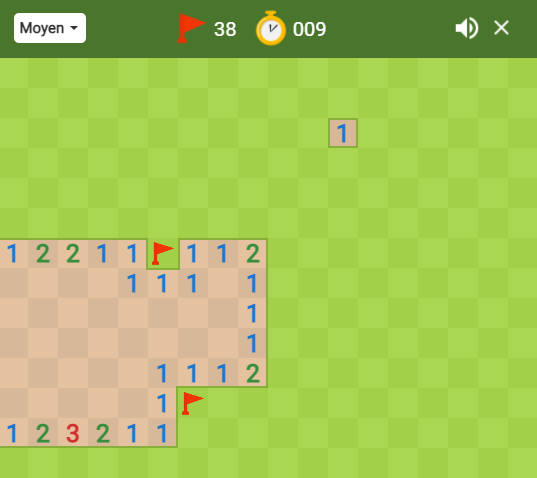
\includegraphics[width=0.577\linewidth]{Ressources/demineurGoogle.png}
    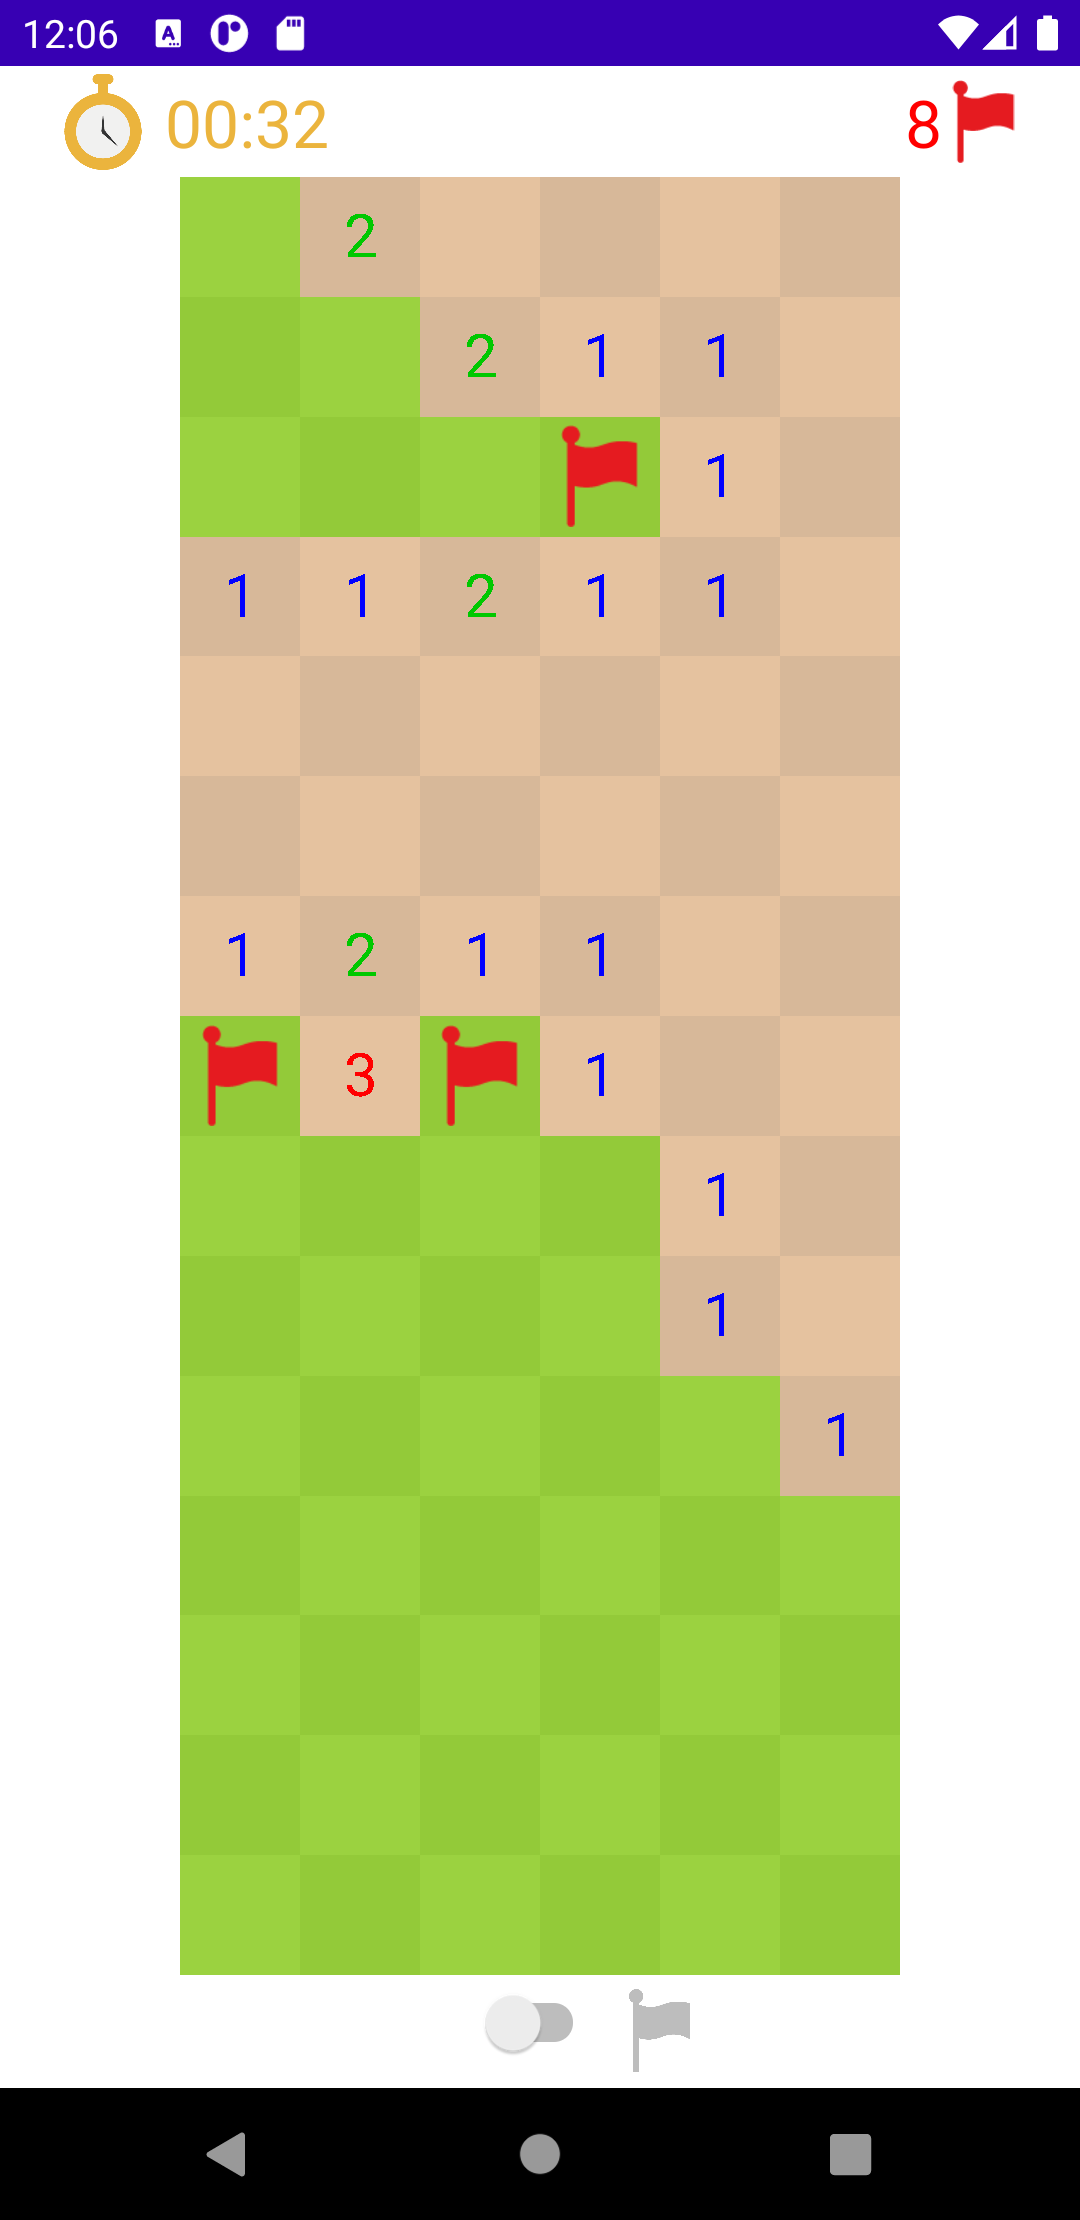
\includegraphics[width=0.25\linewidth]{Ressources/GameplayAndroid.png}
    \caption{A gauche le démineur de Google, à droite le Super Démineur}
  \end{figure}
\end{frame}


\begin{frame}
  \frametitle{Algorithme de creusage}
  \begin{algorithm}[H]
	\KwIn{$c_{i,j}$ la case à creuser de coordonnées $(i,j)$}
	// Cas de base:\\
	\If{$c_{i,j}$ est une bombe \textbf{ou} possède un drapeau}{
	    \Return{}
	}\uElseIf{$c_{i,j}$ a des bombes dans son voisinage de Moore d'ordre 1 }{
	    ouvrir($c_{i,j}$)\\
	    \Return{}
	}
	// Cas récursif: C'est une case vide\\
	ouvrir($c_{i,j}$)\\
	// Creuser les cases dans son voisinage de Von Neuman\\
	\If{$c_{i-1,j}$ est dans la grille}{
	    Creuser($c_{i-1,j}$)
	}
	\If{$c_{i+1,j}$ est dans la grille}{
	    Creuser($c_{i+1,j}$)
	}
	\If{$c_{i,j-1}$ est dans la grille}{
	    Creuser($c_{i,j-1}$)
	}
	\If{$c_{i,j+1}$ est dans la grille}{
	    Creuser($c_{i,j+1}$)
	}
	\caption{Creuser}
\end{algorithm}

\end{frame}

\begin{frame}
\frametitle{Exemple}
\centering
\foreach \x in {1,...,33} {%
    \includegraphics<\x>[width=0.7\linewidth]{Ressources/algo/\x.png}%
}

\end{frame}

\begin{frame}
  \frametitle{Organisation}
    \begin{figure}[H]
        \centering
        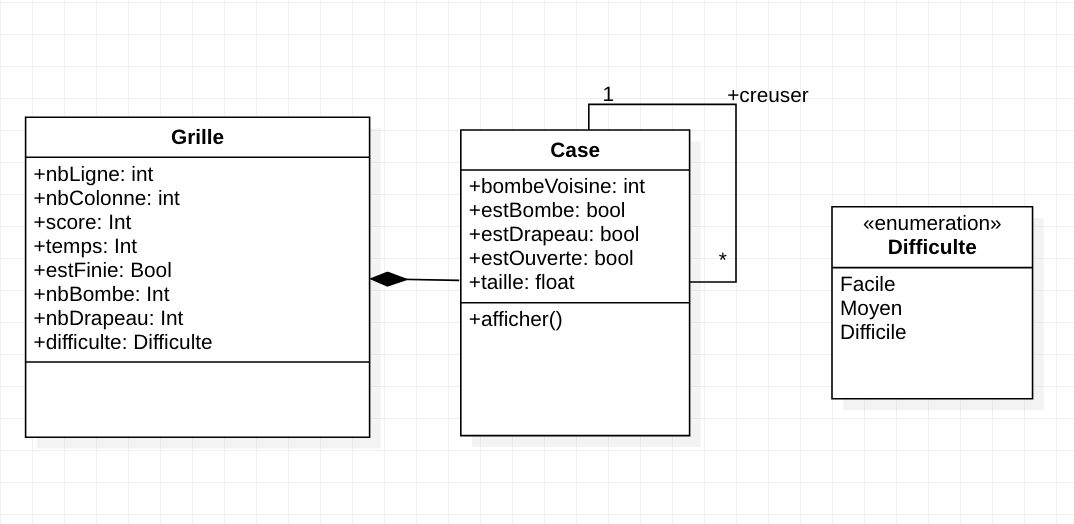
\includegraphics[width=0.6\linewidth]{Ressources/Diagramme_UML.png}
        \caption{Diagramme UML initial}
    \end{figure}
  \begin{itemize}
    \item  la version Android pour Pierre (\url{https://github.com/smallcluster/Demineur})
    \item  la version iOs pour Olivier (\url{https://github.com/Rprojet/Demineur})
  \end{itemize}
\end{frame}



\section{Plateau du jeu}
\subsection{Vue du jeu}

\begin{frame}
  \frametitle{Vue du jeu}
 \begin{figure}[H]
     \centering
      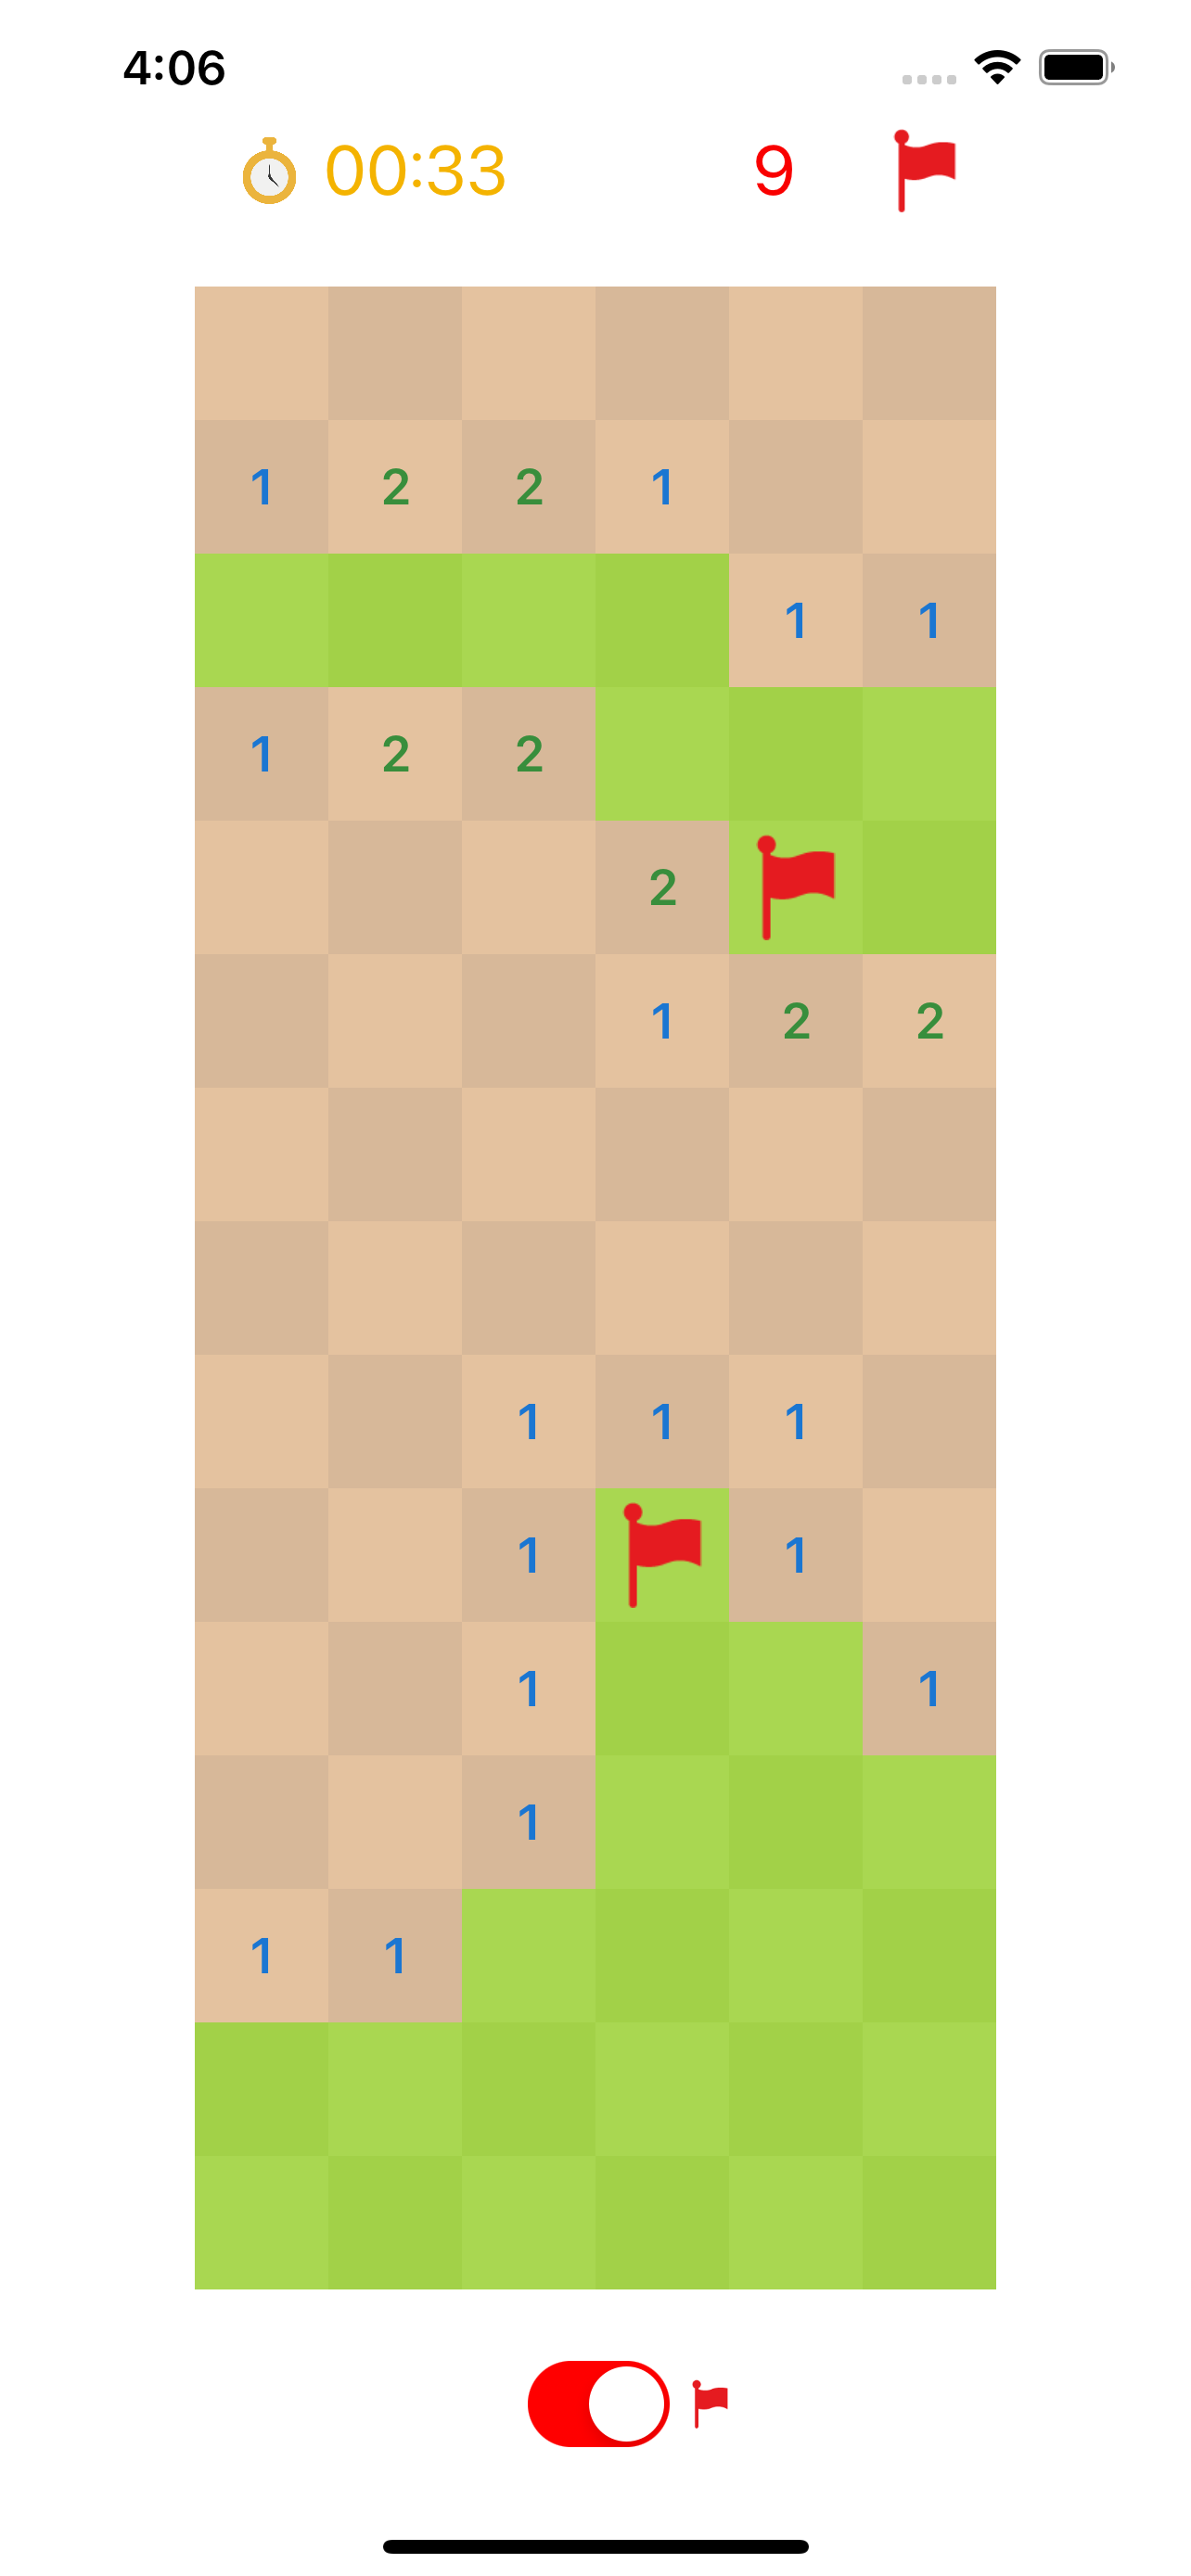
\includegraphics[width=0.25\linewidth]{Ressources/Gameplay_iOs.png}
     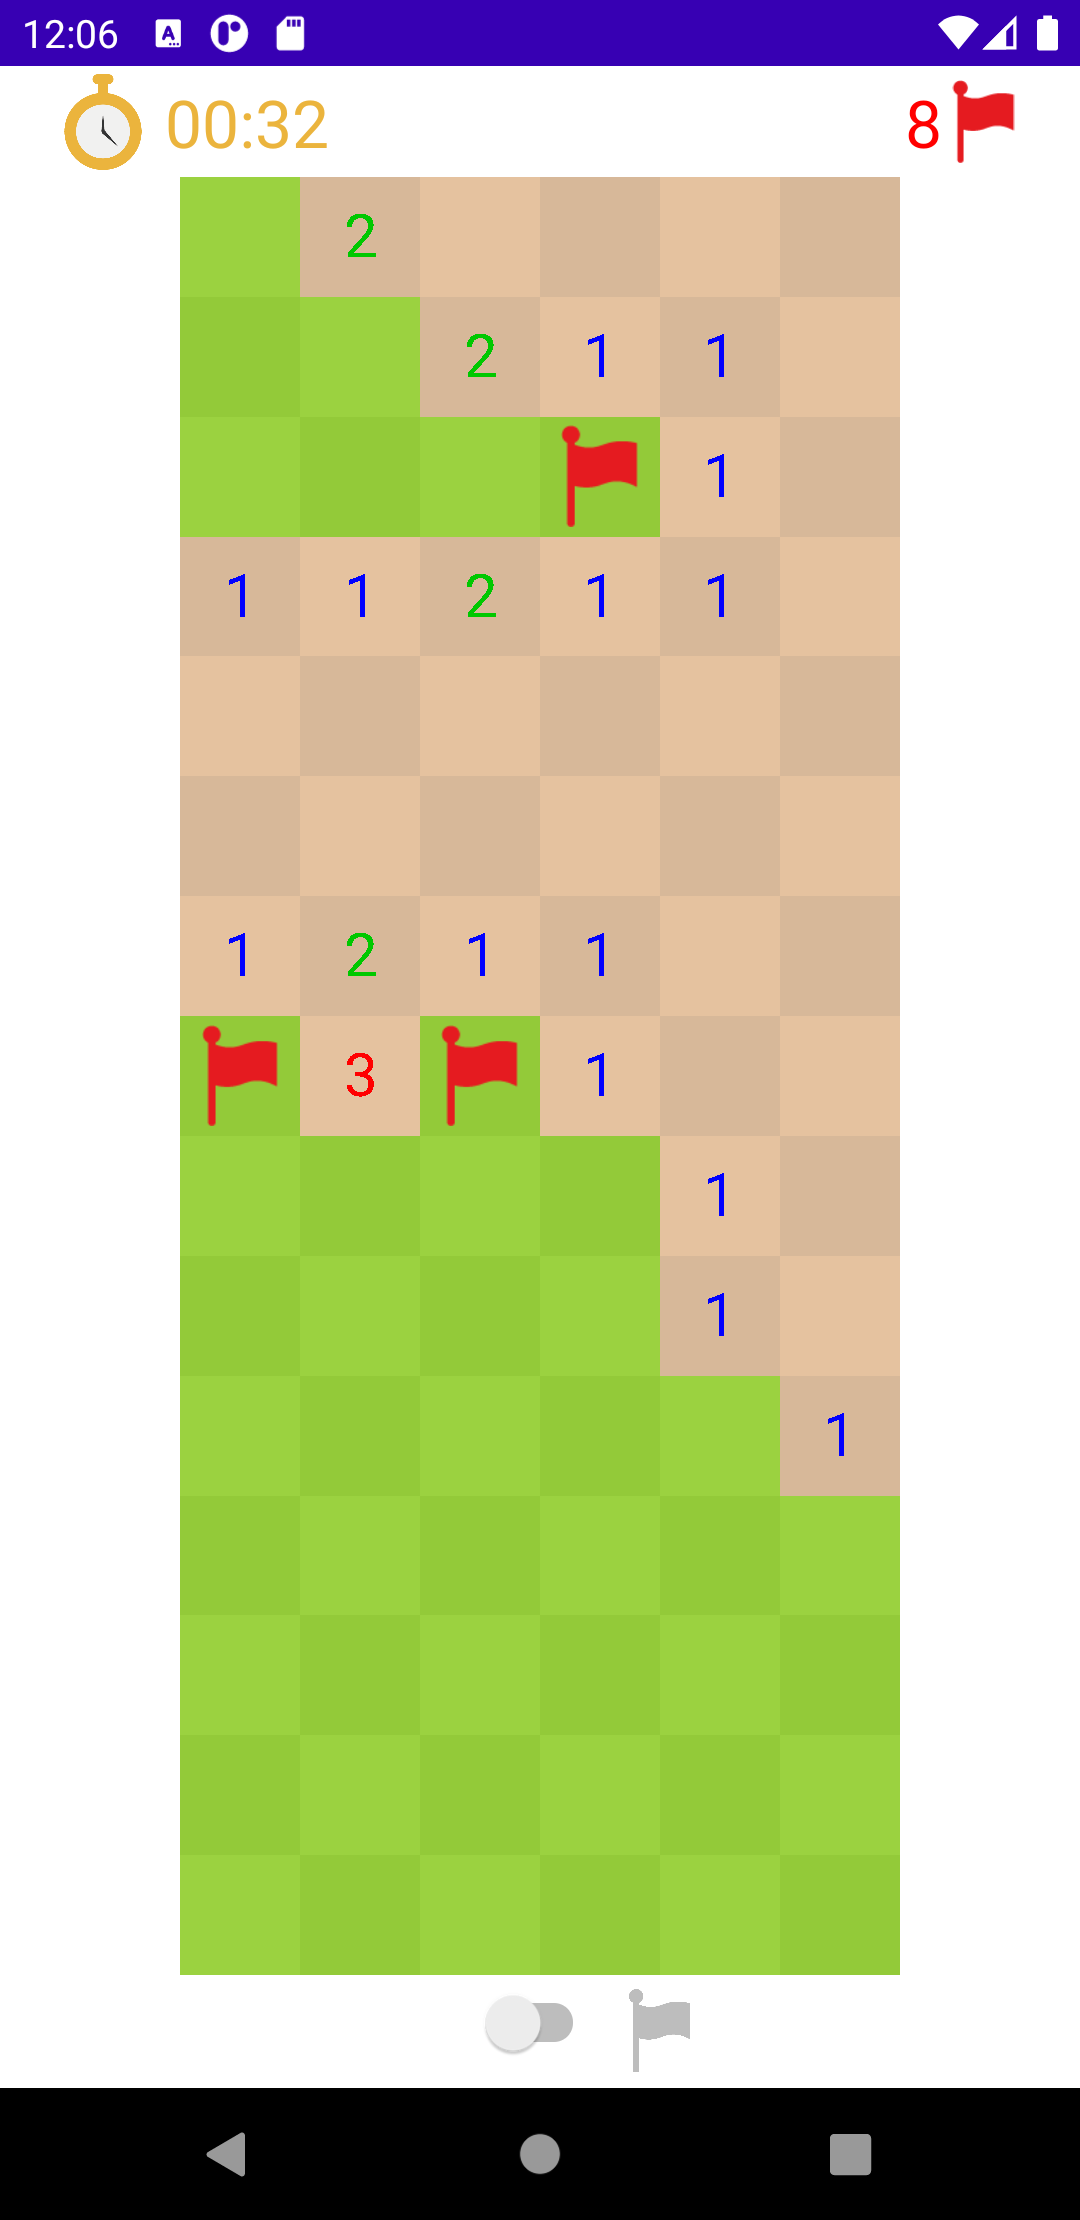
\includegraphics[width=0.25\linewidth]{Ressources/GameplayAndroid.png}
     \caption{Vue du jeu : iOs à gauche, Android à droite}
 \end{figure}
  
\end{frame}

\subsection{Différences iOs/Android}
\begin{frame}
  \frametitle{Différences iOs/Android}
    \framesubtitle{Implémentation}
    \begin{columns}
        \begin{column}{0.4\linewidth}
            \begin{figure}[H]
                \centering
                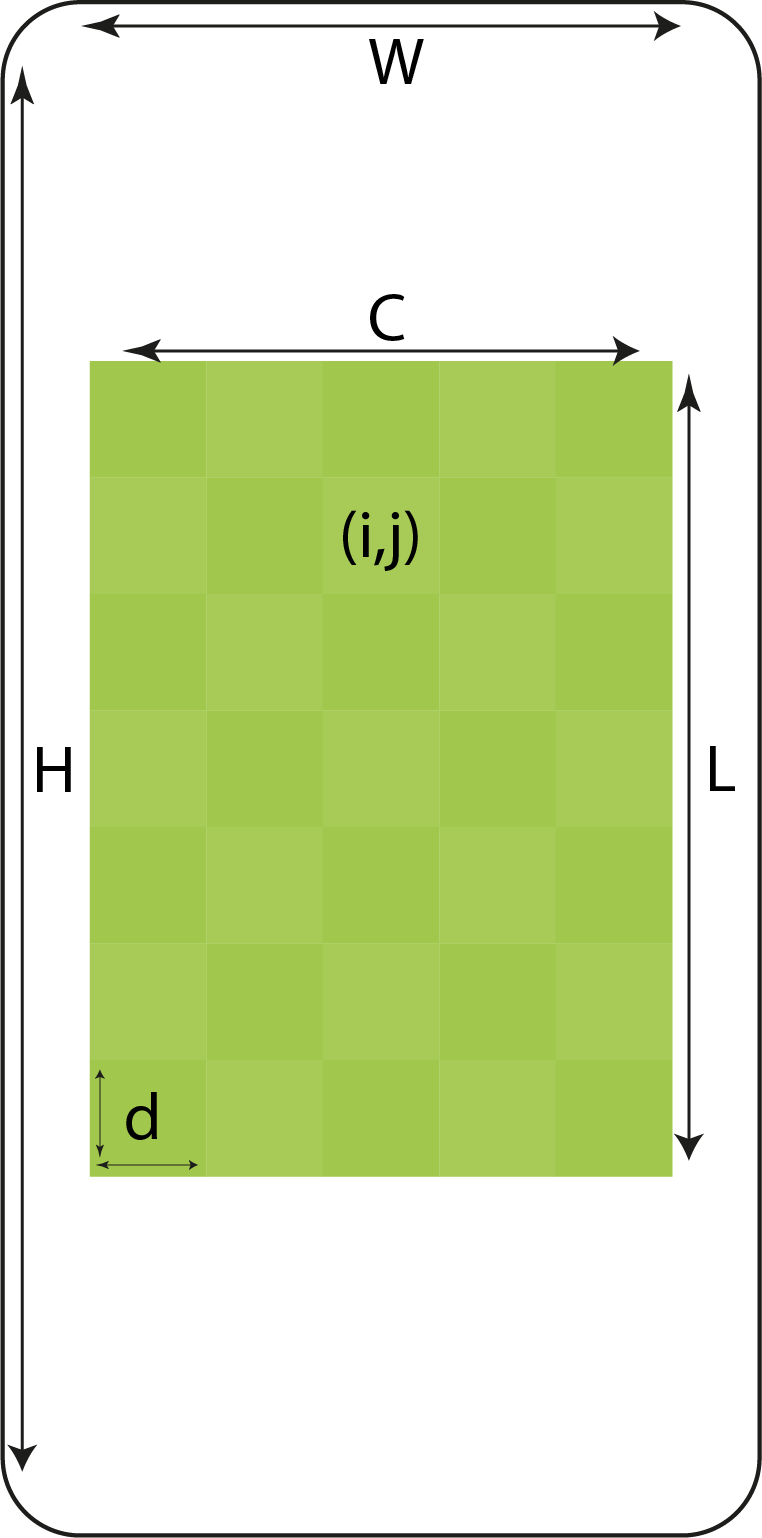
\includegraphics[width=0.5\linewidth]{Ressources/CentrageGrille_iOs.png}
                \caption{iOs}
            \end{figure}
            \tiny
            $$
            \left\{
                \begin{array}{ll}
                    x=i\times d+\frac{(W-c\times d)}{2} \\
                    y=j\times d+\frac{(H-l\times d)}{2}
                \end{array}
            \right.
            $$
        \end{column}
        
        \begin{column}{0.4\linewidth}
            \begin{figure}[H]
                \centering
                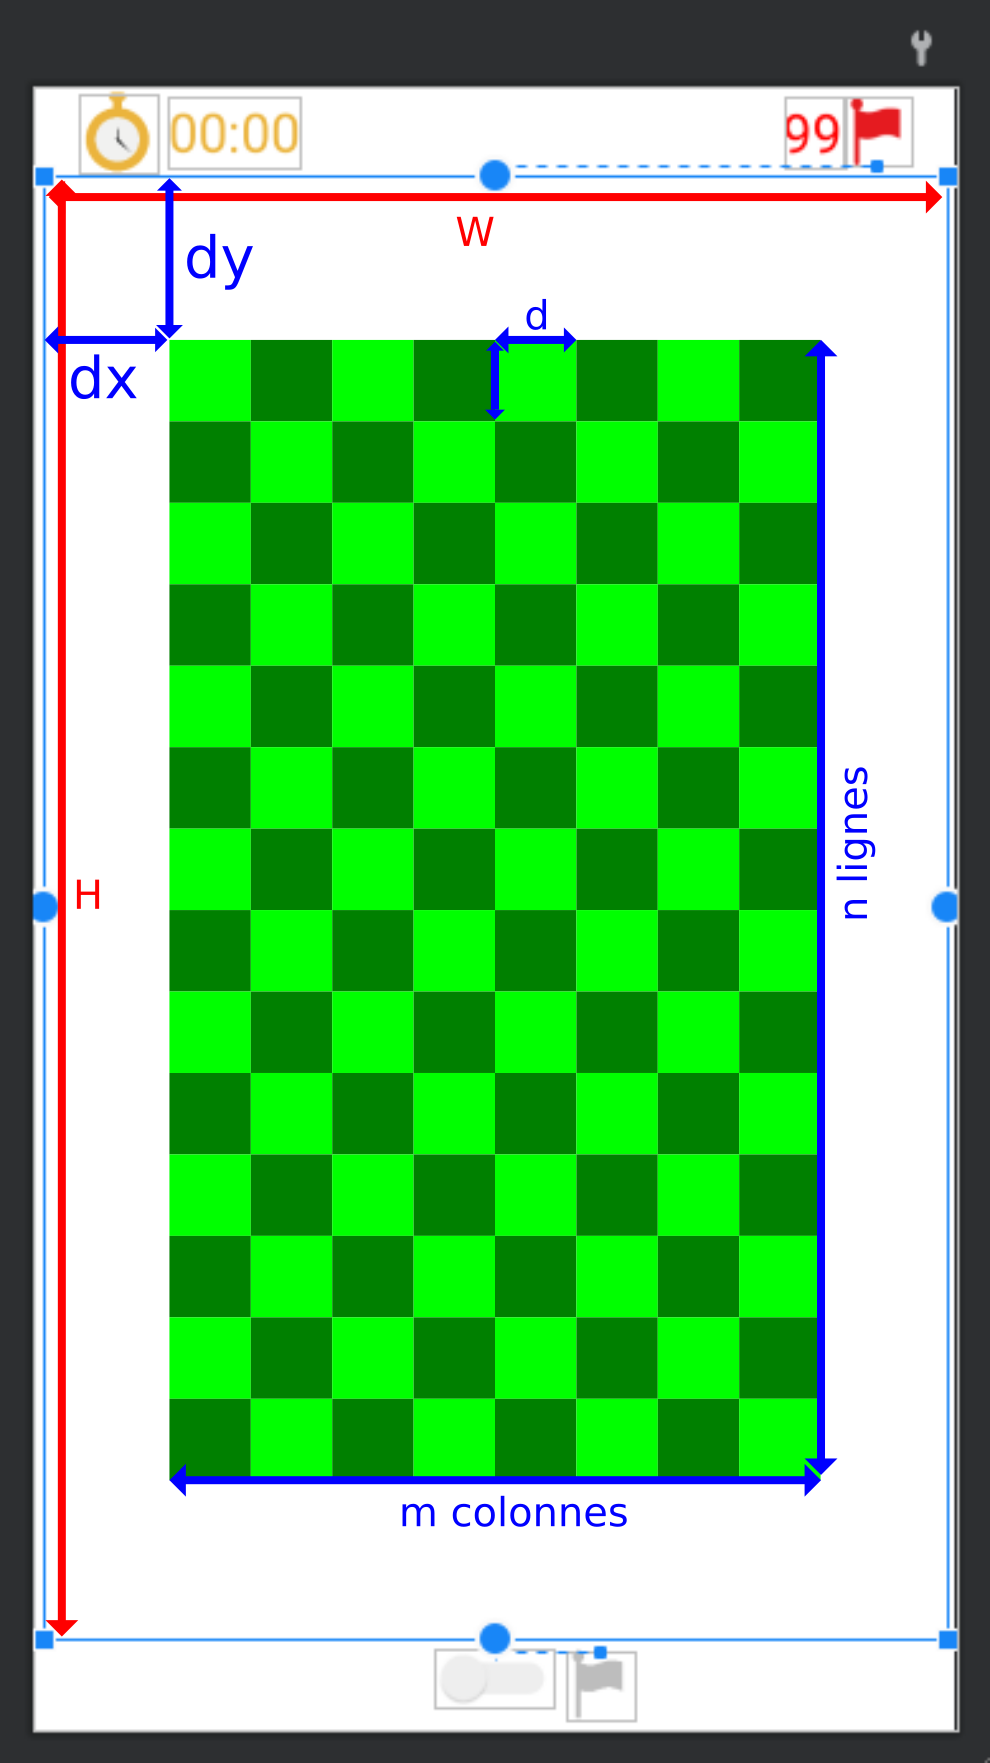
\includegraphics[width=0.57\linewidth]{Ressources/androidPositions.png}
                \caption{Android}
            \end{figure}
            \tiny
            $$
                (x,y) = \begin{dcases}
                    \left( dx+j\times d, dy+i\times d\right) \text{ si mode portrait} \\
                    \left( dx+i\times d, dy+j\times d\right) \text{ si mode paysage}
                \end{dcases}
            $$
            
        \end{column}
    \end{columns}
    
    
    
\end{frame}

\begin{frame}
  \frametitle{Différences iOs/Android}
    \framesubtitle{Taille des cases}
    \centering

    \begin{columns}
    \begin{column}{0.4\linewidth}
    \begin{figure}[H]
    \centering
    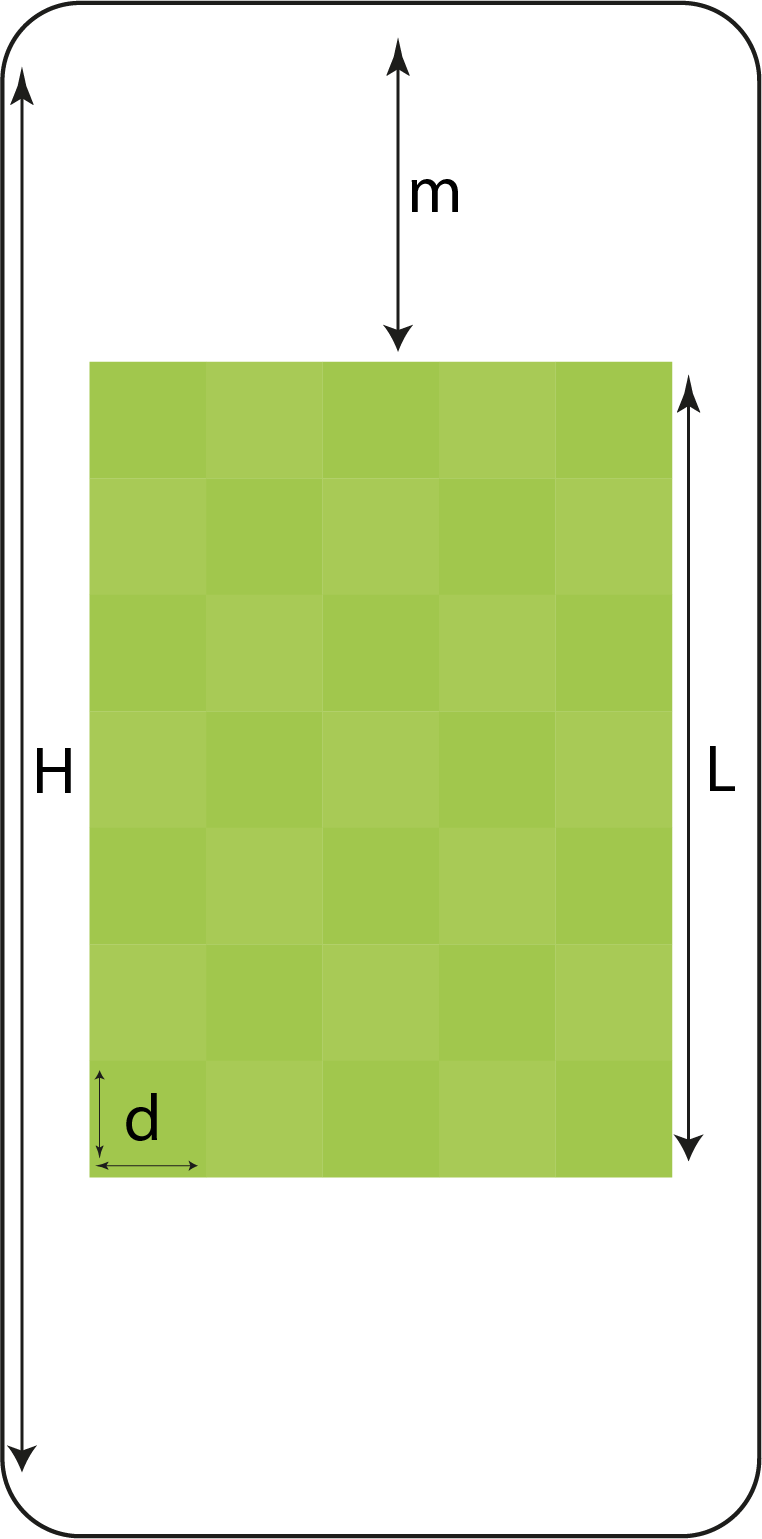
\includegraphics[width=0.5\linewidth]{Ressources/DimensionCase_iOs.png}
    \caption{iOs}
    \end{figure}
    \tiny
    $$d = \frac {(1 - m)\times H }{l}$$
    \end{column}
    \begin{column}{0.4\linewidth}
    \begin{figure}[H]
                \centering
                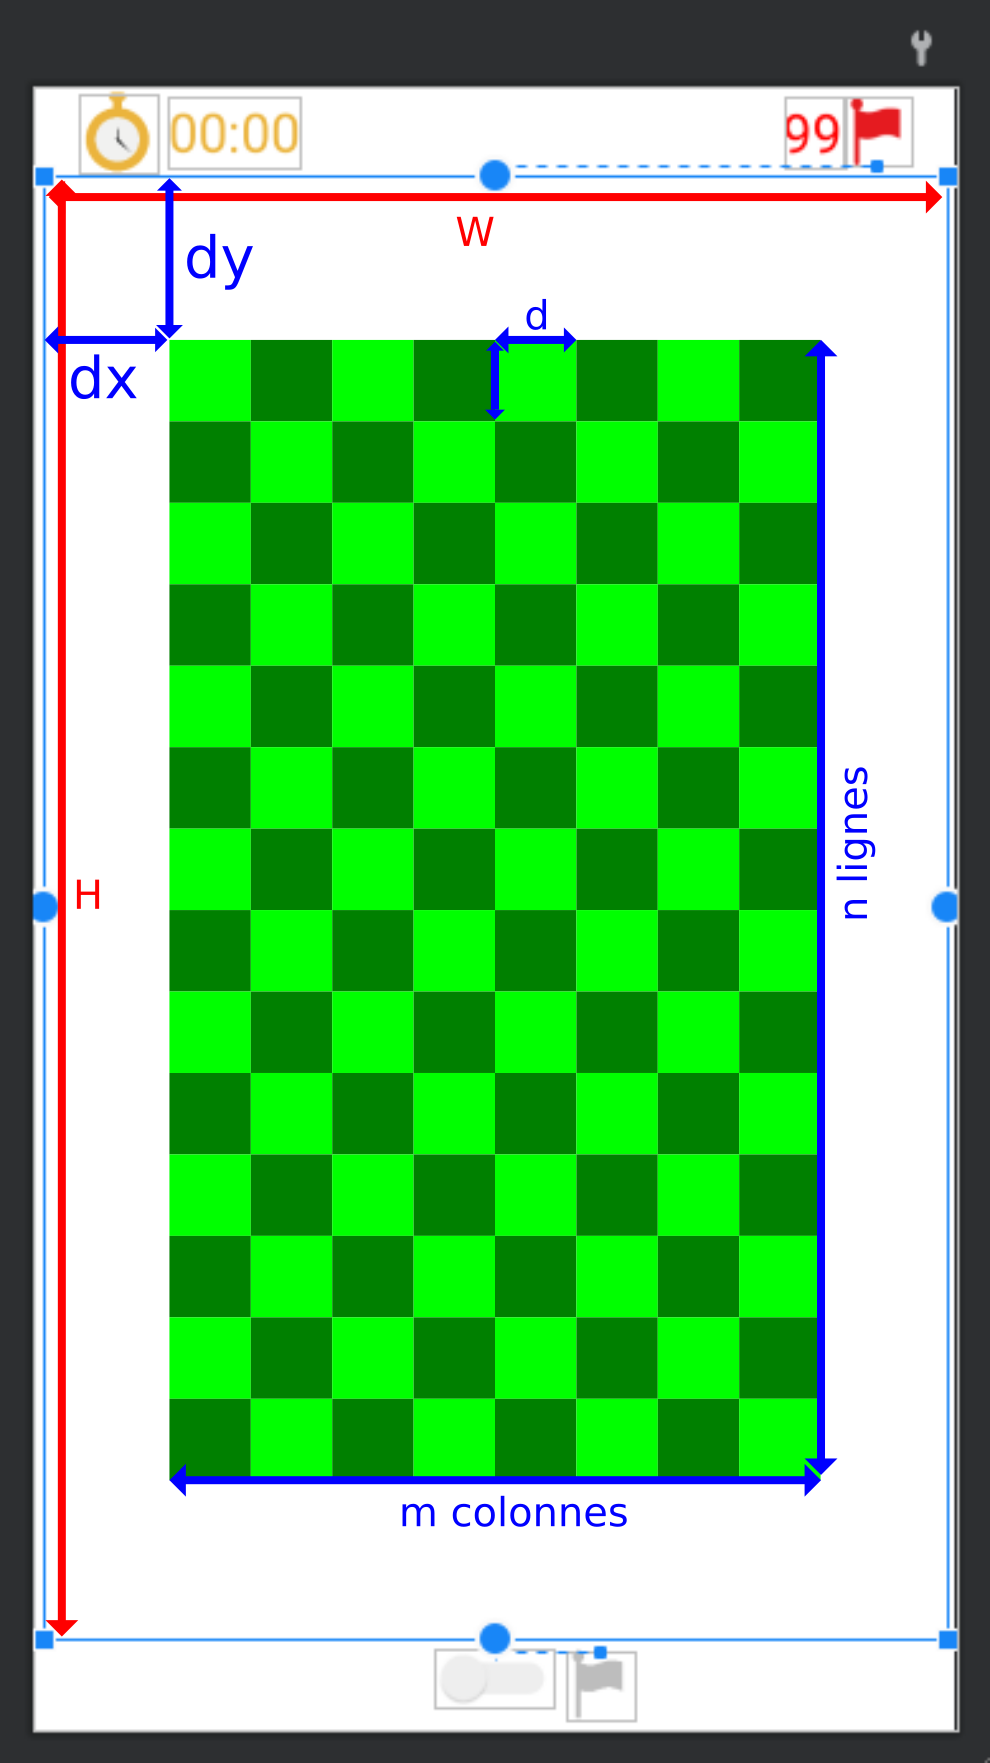
\includegraphics[width=0.5\linewidth]{Ressources/androidPositions.png}
                \caption{Android}
            \end{figure}
            \tiny
            $$d=\begin{dcases}
\Min{}\left(\frac{W}{m}, \frac{H}{n}\right) \text{ si mode portrait} \\
\Min{}\left(\frac{W}{n}, \frac{H}{m}\right) \text{ si mode paysage}
\end{dcases}$$
    \end{column}
    \end{columns}

\end{frame}

\begin{frame}[fragile]
  \frametitle{Différences iOs/Android}
    \framesubtitle{Entrée du joueur}
    
    \begin{columns}
    \begin{column}{0.5\linewidth}
    \noindent \underline{\textit{iOs : Ajout de la callback}}\\
    \begin{minted}[autogobble, breaklines]{swift}
    self.caseBtn.addTarget(self, action:#selector(callback), for:.touchUpInside)
    \end{minted}
    \end{column}
    
    \begin{column}{0.5\linewidth}
    \noindent \underline{\textit{Android : Calcul des coordonnées}}\\
    \tiny
    \begin{minted}[autogobble, breaklines]{java}
float mx = event.getX();
float my = event.getY();
int rotation = display.getRotation();
int tm = Surface.ROTATION_0 != rotation ? n : m;
int tn = Surface.ROTATION_0 != rotation ? m : n;
if(mx < xOffset || mx > xOffset+tailleCase*tm || my < yOffset || my > yOffset+tailleCase*tn)
    return true;
int j = (int) ((mx - xOffset) / tailleCase);
int i = (int) ((my - yOffset) / tailleCase);
if(Surface.ROTATION_0 != rotation){ int tmp=i; i=j; j=tmp;}
    \end{minted}
    \end{column}
    \end{columns}
\end{frame}


\begin{frame}[fragile]
  \frametitle{Différences iOs/Android}
    \framesubtitle{Dialogue entre les vues}
    
    \begin{columns}
    
    \begin{column}{0.5\linewidth}
    \tiny
    \begin{figure}[H]
    
            \begin{tikzpicture}
            \sbEntree{E}
            \sbBlocr[7]{r2}{MainViewController}{E}
            \sbBlocr[5]{r3}{ScoreViewController}{r2}
            \sbRelier[ShowScore]{r2}{r3}
            \end{tikzpicture}
            \caption{Diagramme vue/segue}
    \end{figure}
    \begin{minted}[autogobble]{swift}
override func prepare(for segue: UIStoryboardSegue, 
sender: Any?) 
{
    if segue.identifier == "ShowScore"
    {
        let VCDestination = segue.destination as! 
        ScoreViewController

        VCDestination.fillDataTabView(scoreList)
    }
}
    \end{minted}
    
    \end{column}
    
    \begin{column}{0.5\linewidth}
    \tiny
    \begin{figure}[H]
            \begin{tikzpicture}
            \sbEntree{E}
            \sbBlocr[7]{r2}{MainActivity}{E}
            \sbBlocr[5]{r3}{ScoresActivity}{r2}
            \sbRelier[voirScores]{r2}{r3}
            \end{tikzpicture}
            \caption{Diagramme activity/intent}
    \end{figure}
    \begin{minted}[autogobble]{java}
public void voirScores(View v){
    Intent intent=new Intent(this,ScoresActivity.class);
    intent.putStringArrayListExtra("array", stats); 
    startActivity(intent);
}
    \end{minted}
    \end{column}
    \end{columns}
    
\end{frame}


\begin{frame}
  \frametitle{Différences iOs/Android}
    \framesubtitle{Liste de score}
    \begin{figure}
        \centering
        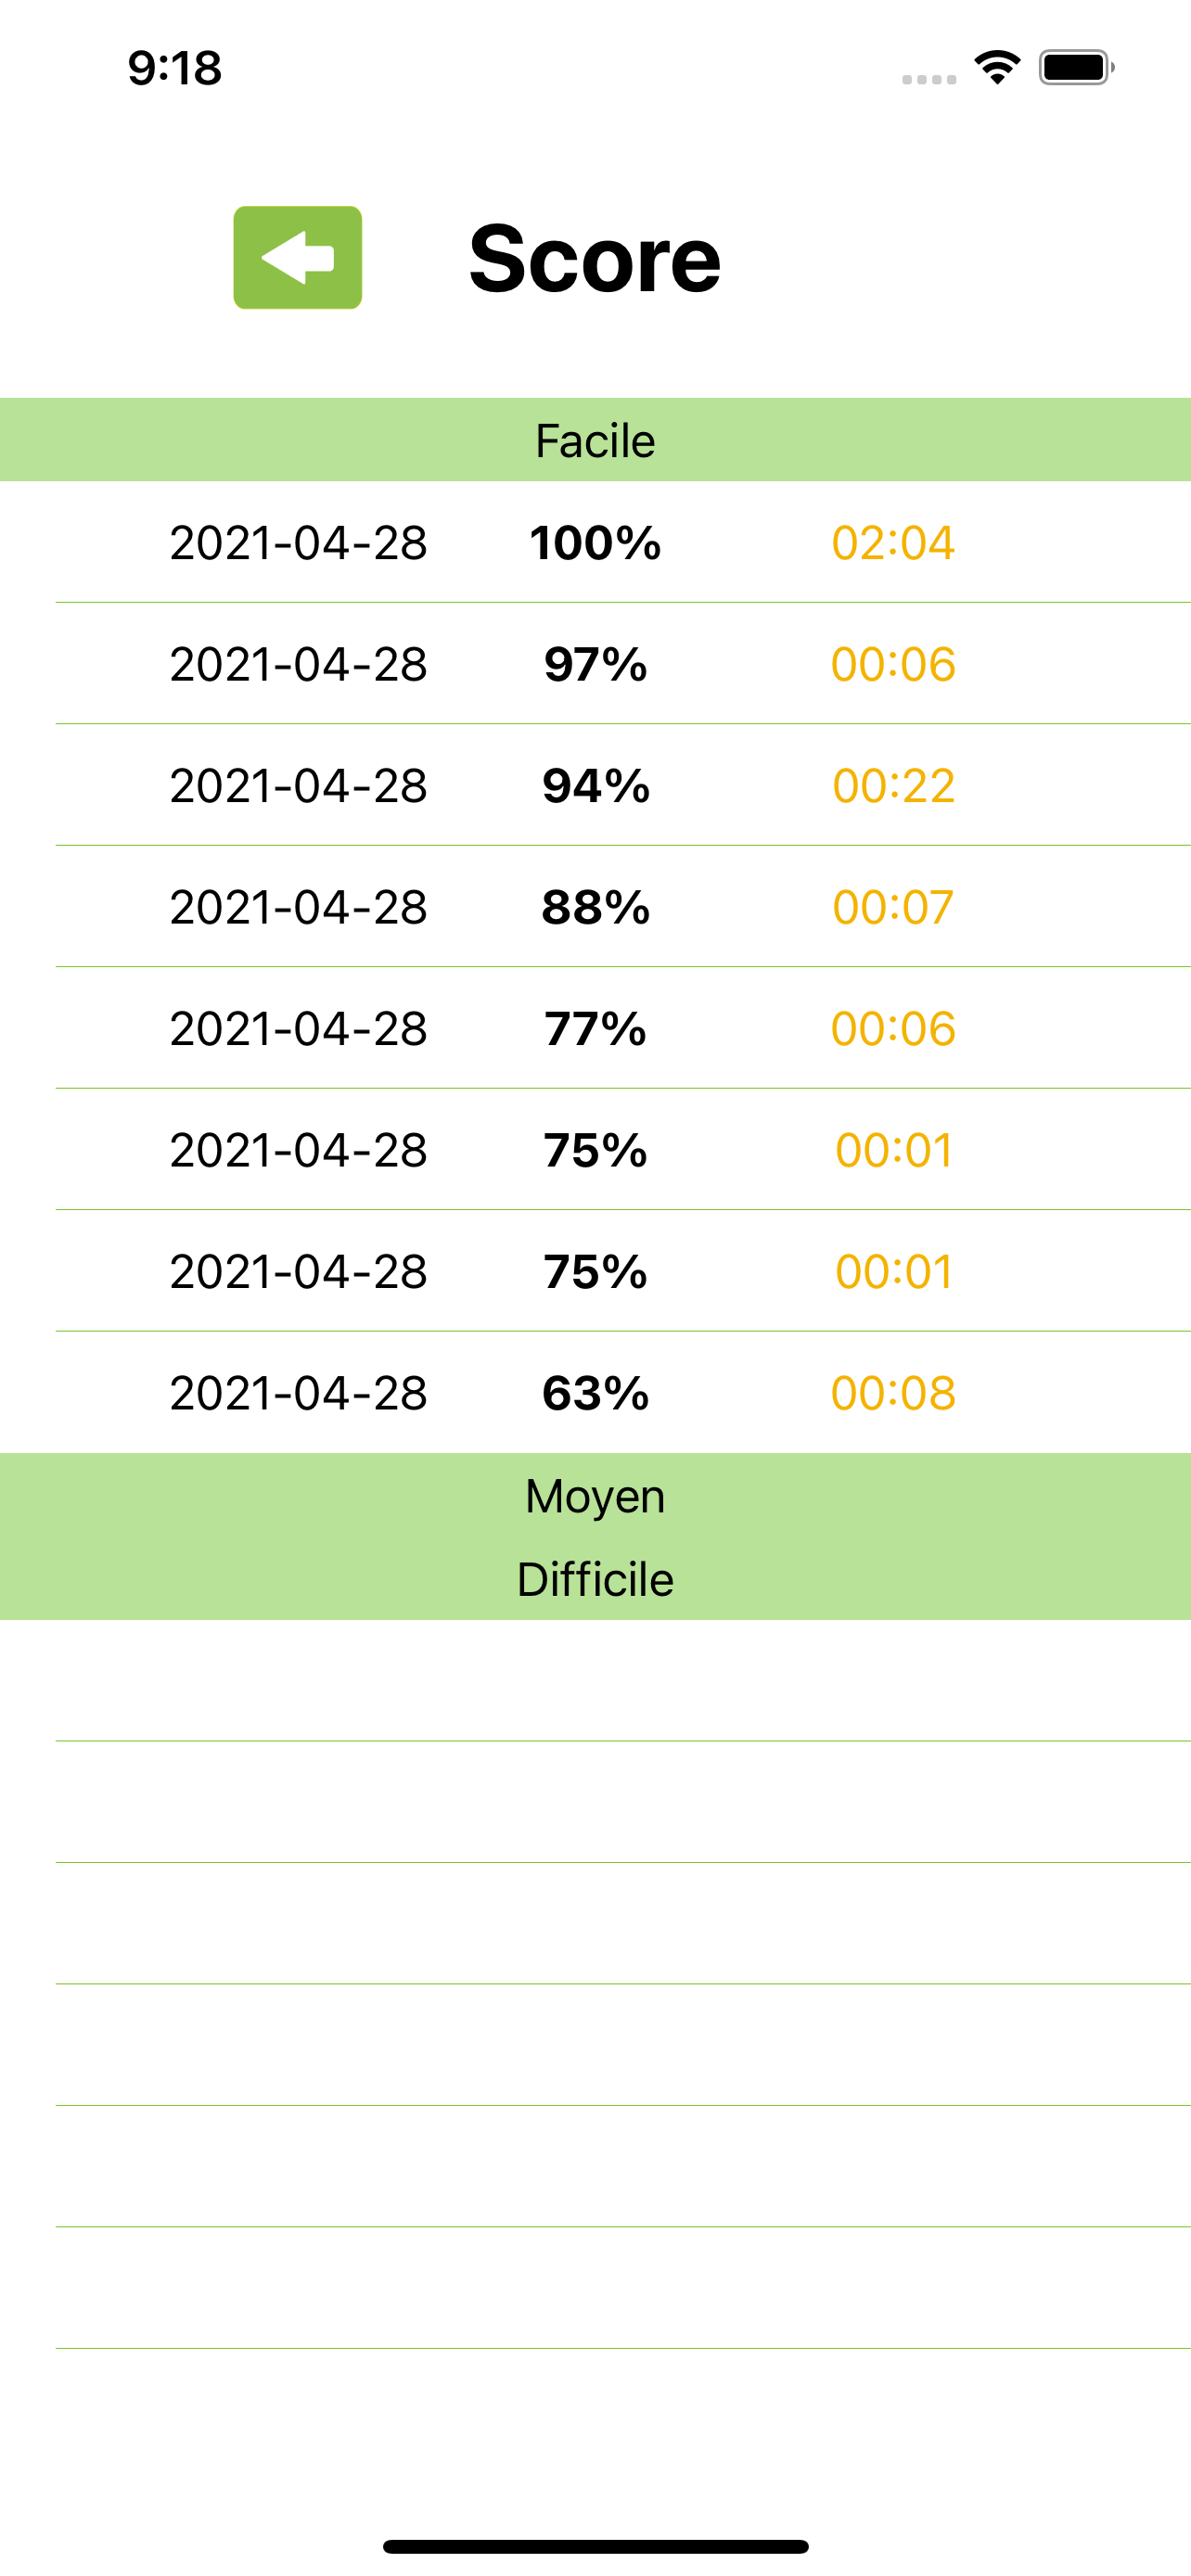
\includegraphics[width=0.23\linewidth]{Ressources/ScoreView_iOs.png}
        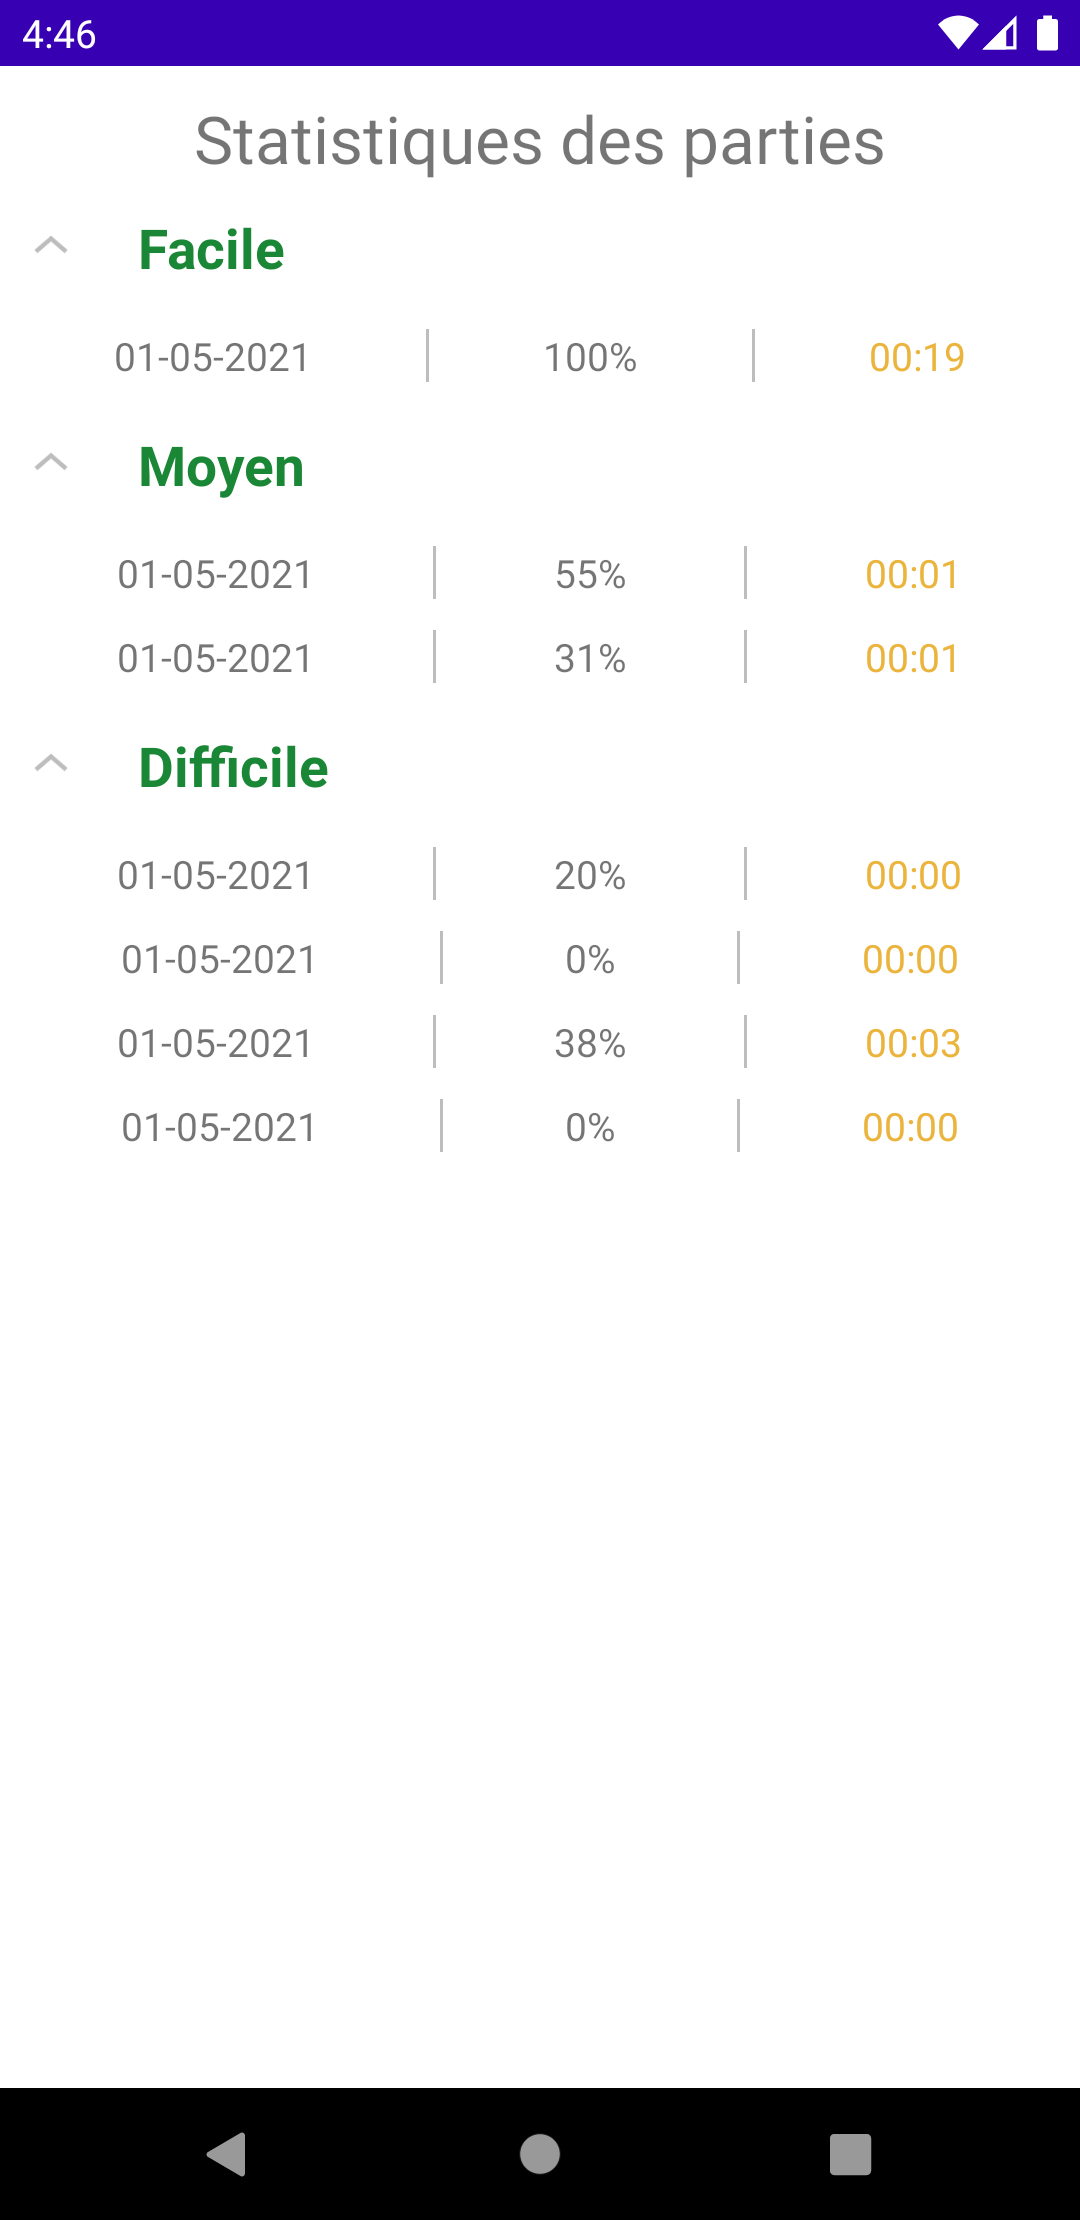
\includegraphics[width=0.23\linewidth]{Ressources/androidListView.png}
        \caption{Historique des scores : iOs à gauche, Android à droite}
    \end{figure}
\end{frame}


\begin{frame}[fragile]
  \frametitle{Différences iOs/Android}
    \framesubtitle{Persistance des données}

    \begin{columns}
    \tiny
        \begin{column}{0.5\linewidth}
        \begin{figure}[H]
            \centering
            \includegraphics[width=1\linewidth]{Ressources/Persistance_Donnée_iOs.png}
            \caption{iOs : Processus persistance}
        \end{figure}
        \end{column}
        
        \begin{column}{0.5\linewidth}
            \begin{figure}[H]
            \centering
            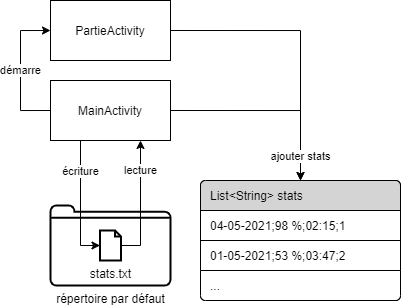
\includegraphics[width=1\linewidth]{Ressources/dataAndroid.png}
            \caption{Android : modification de l'historique}
        \end{figure}
        \end{column}
    \end{columns}
\end{frame}

\begin{frame}
  \frametitle{Différences iOs/Android}
  \framesubtitle{Synthèse}
  \begin{tabular}{|r|l|c|}
  \hline
      & iOs & Android\\
  \hline
      Implémentation & UIButton & Canvas \\
      Taille des cases  &  \% hauteur écran & remplissage maximum  \\
      Entrée du joueur  & Callback & onTouchListener  \\
      Dialogue entre les vues  & Segue & Intent  \\
      Liste de score  & UITableView & ExpendableListView  \\
      Persistance des données  & UserDefaults & text file  \\
  \hline
\end{tabular}

  
  % 6 min
\end{frame}



\section{Conclusion}

\begin{frame}
  \frametitle{Conclusion}
  \begin{itemize}
    \item communiquer entre membres pour imposer des limites réalistes et garder une interface graphique homogène entre iOs et Android
    \item découvrir les mécaniques qui régissent le jeu du démineur
    \item comparer l' implémentation native entre iOs et Android \\
\end{itemize}

\end{frame}

\section{Démonstration}

\end{document}